\documentclass[tikz,border=8pt]{standalone}
\usepackage{amsmath,amssymb}
\usetikzlibrary{arrows.meta,calc}

\begin{document}
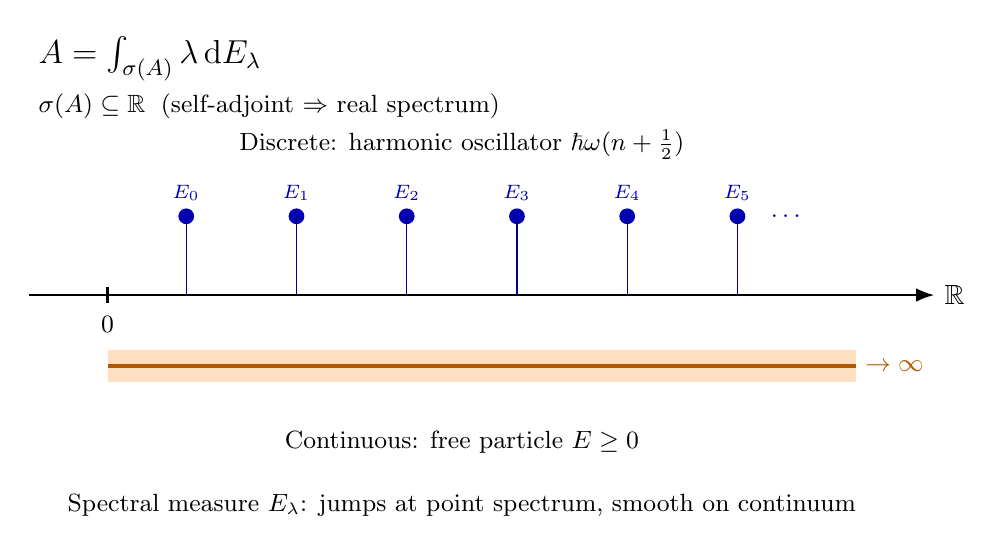
\begin{tikzpicture}[>=Latex]

  % main horizontal real axis
  \draw[->, thick] (-1, 0) -- (10.5, 0) node[right]{$\mathbb R$};
  \draw[thick] (0, -0.1) -- (0, 0.1);
  \node[font=\small, anchor=north] at (0, -0.15) {$0$};

  % Discrete spectrum (above): harmonic oscillator
  \node[font=\small, anchor=south] at (4.5, 1.6) {Discrete: harmonic oscillator $\hbar\omega(n+\tfrac12)$};
  \foreach \x/\n in {1.0/0, 2.4/1, 3.8/2, 5.2/3, 6.6/4, 8.0/5}{
    \fill[blue!70!black] (\x, 1.0) circle (0.10);
    \draw[thin, blue!50!black] (\x, 1.0) -- (\x, 0);
    \node[font=\scriptsize, blue!70!black, anchor=south] at (\x, 1.07) {$E_\n$};
  }
  \node[font=\small, blue!70!black, anchor=west] at (8.3, 1.0) {$\dots$};

  % Continuous spectrum (below): free particle
  \node[font=\small, anchor=north] at (4.5, -1.6) {Continuous: free particle $E\ge 0$};
  \fill[orange!50, opacity=0.5] (0, -1.1) rectangle (9.5, -0.7);
  \draw[very thick, orange!70!black] (0, -0.9) -- (9.5, -0.9);
  \node[font=\small, orange!70!black, anchor=west] at (9.5, -0.9) {$\to\infty$};

  % top formula
  \node[font=\large, anchor=west] at (-1, 3.0) {$A=\int_{\sigma(A)}\lambda\,\mathrm dE_\lambda$};
  \node[font=\small, anchor=west] at (-1, 2.4) {$\sigma(A)\subseteq\mathbb R$ \;(self-adjoint $\Rightarrow$ real spectrum)};

  % bottom note
  \node[font=\small, anchor=north] at (4.5, -2.4) {Spectral measure $E_\lambda$: jumps at point spectrum, smooth on continuum};
\end{tikzpicture}
\end{document}
